
For the train models we provide the resulting metrics on the downstream tasks. In this case only two metrics are important for evaluation --- cell area and cell count (see Table \ref{table:gfp-metrics}). Both Pearson correlation and Spearman rank coefficients are lower than in previous experiments. Influence of additional segmentation of dead cells by the model lowers correlation scores, however they still signalize the presence of strong correlation between prediction and ground truth.
\begin{table}[H]
    \centering
    \caption{Correlation coefficients for downstream tasks}
        \begin{adjustbox}{width=0.4\textwidth}
            \begin{tabular}{|c|c|c|}\hline
                BCE loss&Pearson&Spearman
                \\\hline\hline
                Number of ER&0.67&0.64\\\hline
                Area&0.82&0.75\\\hline
            \end{tabular}
            \label{table:gfp-metrics}
        \end{adjustbox}
\end{table}

Violin and scattter plots depicting two metrics mentioned above are presented in Figure \ref{fig:gfp-bce-metrics}.
\begin{figure}[H]
	\begin{center}
		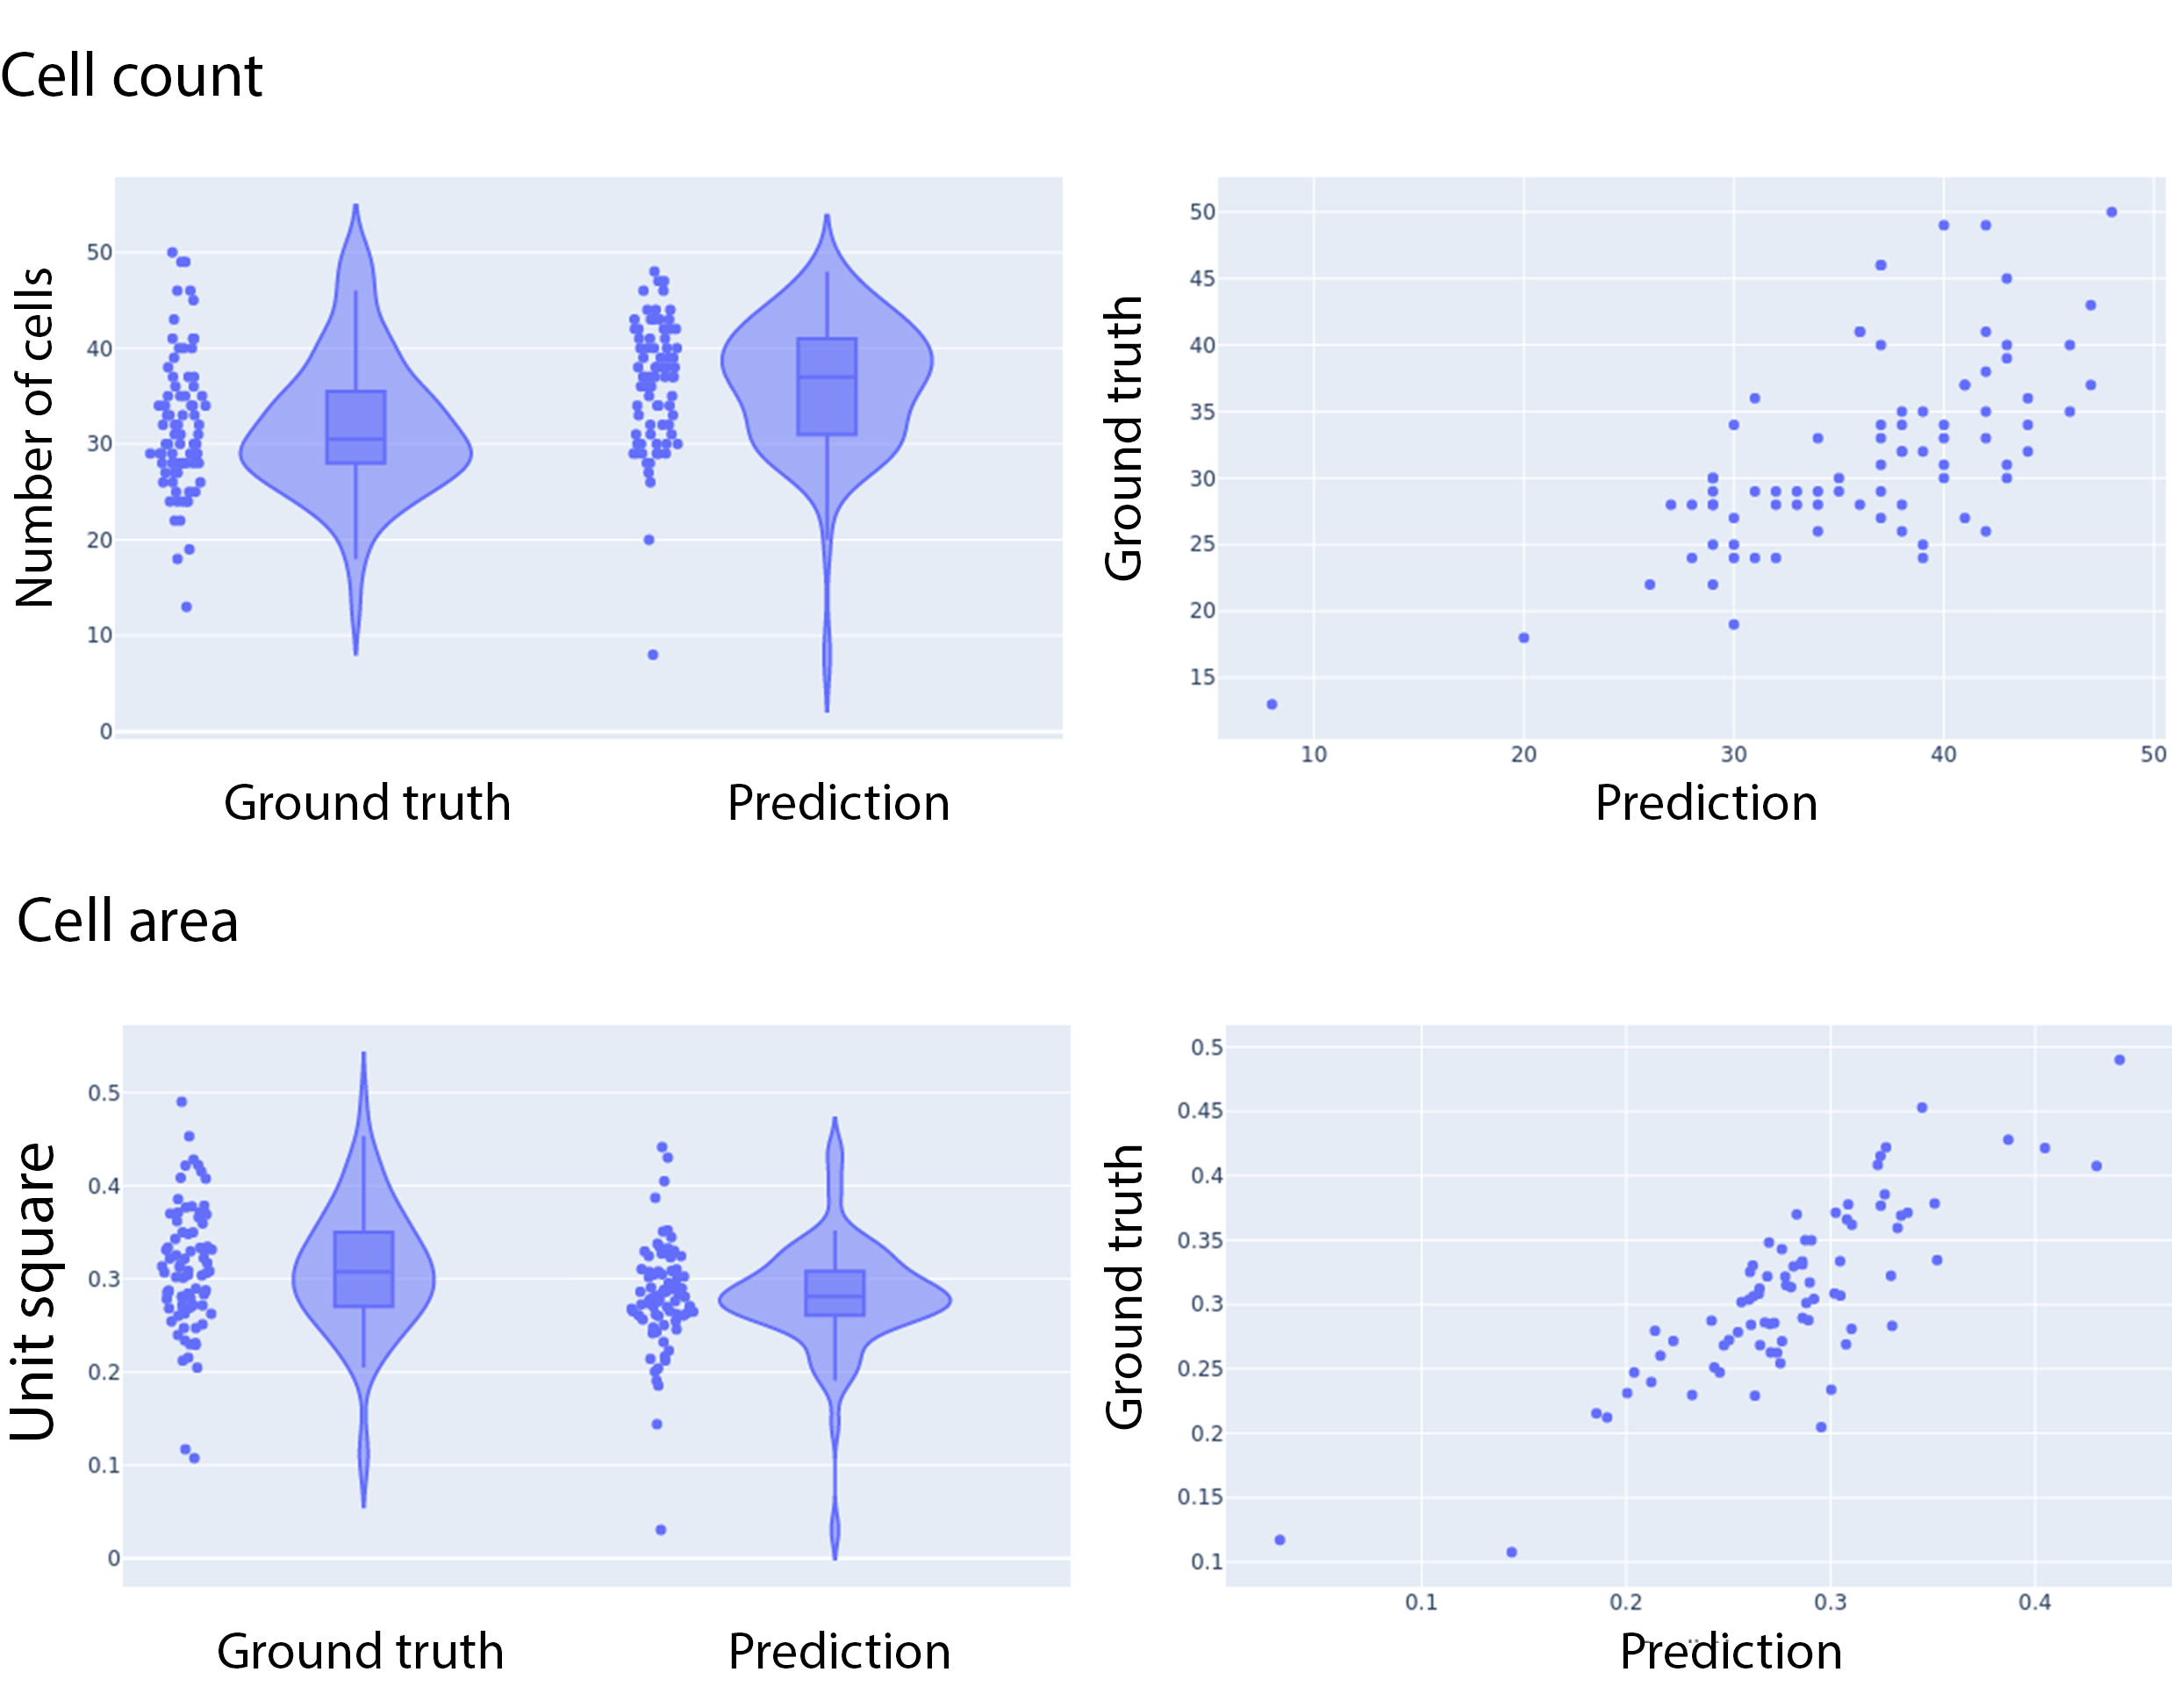
\includegraphics[width=\linewidth]{bilder/gfp/binary-bce/gfp-bce-metrics.png}
		\caption{Downstream metrics}\label{fig:gfp-bce-metrics}
	\end{center}
\end{figure}
